\documentclass[fleqn,10pt]{wlscirep}
\usepackage[utf8]{inputenc}
\usepackage[T1]{fontenc}
\title{NANSNA: Improving Neuromorphic Computing Efficiency with Neuromorphic Accelerators with Novel Spiking Neural Subnetwork Ensemble-Based Architecture}

\author[1,*]{Dean Jordan}
\author[2]{Bob Author}
\author[1,2,+]{Christine Author}
\author[2,+]{Derek Author}
\affil[1]{University of Michigan, Artificial Intelligence, South Lyon, 48178, United States}
\affil[2]{Affiliation, department, city, postcode, country}

\affil[*]{jordan.dean161@gmail.com}

\affil[+]{these authors contributed equally to this work}

%\keywords{Keyword1, Keyword2, Keyword3}

\begin{abstract}
As a field, neuromorphic computing is expected to nearly double annually until 2032 and have an expected valuation of \$9.5 trillion USD. However, current implementations of neuromorphic accelerators contains models which are not large enough for Vision and Language (VaL) tasks and are relatively incapable of multi-domain learning due to the specialization of current Spiking Neural Network (SNN) architectures. As a result, the NANSNA architecture aims to improve the efficiency of SNNs by developing a novel encoder/decoder-based SNN architecture which utilizes a neural subnetwork ensemble. The architecture contains multiple novel neuron and layer types within the central subnetwork for increasing efficiency, specialization, and multi-domain learning. Additional efficiency improvements occur due to the encoder and decoder being non-spiking. The NANSNA model is trained on an adapter-based approach. Each subnetwork in the subnetwork ensemble is assigned a single adapter. This allows for specialization to occur while simultaneously increasing the performance of multi-domain tasks. Finally, NANSNA is converted to an open source neuromorphic accelerator, further improving efficiency. The NANSNA model and architecture demonstrate statistically significant improvement in several key metrics within neuromorphic computing, including Synaptic Operations per Second (SOPS), synaptic density, Neuromorphic MNIST (N-MNIST), and the cost per neuron.
\end{abstract}
\begin{document}

\flushbottom
\maketitle
% * <john.hammersley@gmail.com> 2015-02-09T12:07:31.197Z:
%
%  Click the title above to edit the author information and abstract
%
\thispagestyle{empty}

\section*{Introduction}

Artificial Neural Networks (ANNs) are a firmly established state of the art method in machine learning. The artificial neuron converts an input tensor to an output tensor via a linear transformation combined with a nonlinear activation function. Due to this methodology, several state of the art machine learning architectures such as the Recurrent Neural Network (RNN) and Transformer have developed. A majority of the architectures developed from ANNs have drawn similarities from the field of neuroscience. However, despite the arrival of novel machine learning architectures, balancing specialization alongside multi-domain performance and efficiency has proven to be a major challenge of researchers within Machine Learning (ML). Thus, the SNN was proposed as a novel paradigm separate from ANNs. While ANNs utilize continuous-valued outputs, SNNs intend to utilize action potentials to convert an input tensor into an output tensor.

The resulting architecture, while significantly improving the specialization and single-domain performance of neural networks, underperforms in multi-domain performance due to SNNs containing a temporal dimension. Additionally, due to the complexity of the temporal dimension, a majority of SNNs have few model parameters as compared to ANNs. Though neuromorphic accelerators have since been proposed to partially mitigate this, current architectures based on SNNs are nevertheless less efficient than ANNs and, as a result of being composed fully of spiking neurons, would continue to suffer from low efficiency despite being adopted into neuromorphic accelerators. Thus, the synaptic density of a typical neuromorphic accelerator limits the use cases of SNNs. As such, neuromorphic accelerators based on current SNN architectures are generally computationally expensive and the cost per neuron is typically significantly more substantial than the cost of current methods of software-based ANNs combined with hardware accelerators.

As such, this report proposes a novel SNN architecture, model, and neuromorphic accelerator intended to provide state of the art performance in multi-domain learning while improving the synaptic density and efficiency of neuromorphic accelerators. The architecture, NANSNA, is based on an encoder-decoder structure with a multi-head attention mechanism, positional encoding mechanism, and recurrent network on both the encoder and decoder. In between the encoder and decoder, a subnetwork ensemble based on residual connections is used. The subnetwork ensemble, unlike the encoder and decoder, is spiking and uses an adapter-based training method in order to achieve parameter efficiency. Each subnetwork within the subnetwork ensemble utilizes a single adapter to allow for multiple adapters to be utilized simultaneously, allowing for multi-domain performance to occur while maintaining specialization and efficiency. Finally, the recurrent network within the encoder utilizes neurosymbolic programming primitives in order to dynamically load adapters according to the input received. Thus, the NANSNA model utilizes multimodality, allowing for the model and architecture to perform competitively to current state of the art ANNs.

\section*{Background}

Neuromorphic computing 

\section*{Results}

Up to three levels of \textbf{subheading} are permitted. Subheadings should not be numbered.

\subsection*{Subsection}

Example text under a subsection. Bulleted lists may be used where appropriate, e.g.

\begin{itemize}
\item First item
\item Second item
\end{itemize}

\subsubsection*{Third-level section}
 
Topical subheadings are allowed.

\section*{Discussion}

The Discussion should be succinct and must not contain subheadings.

\section*{Methods}

Topical subheadings are allowed. Authors must ensure that their Methods section includes adequate experimental and characterization data necessary for others in the field to reproduce their work.

\bibliography{sample}

\noindent LaTeX formats citations and references automatically using the bibliography records in your .bib file, which you can edit via the project menu. Use the cite command for an inline citation, e.g.  \cite{Hao:gidmaps:2014}.

For data citations of datasets uploaded to e.g. \emph{figshare}, please use the \verb|howpublished| option in the bib entry to specify the platform and the link, as in the \verb|Hao:gidmaps:2014| example in the sample bibliography file.

\section*{Acknowledgements (not compulsory)}

Acknowledgements should be brief, and should not include thanks to anonymous referees and editors, or effusive comments. Grant or contribution numbers may be acknowledged.

\section*{Author contributions statement}

Must include all authors, identified by initials, for example:
A.A. conceived the experiment(s),  A.A. and B.A. conducted the experiment(s), C.A. and D.A. analysed the results.  All authors reviewed the manuscript. 

\section*{Additional information}

To include, in this order: \textbf{Accession codes} (where applicable); \textbf{Competing interests} (mandatory statement). 

The corresponding author is responsible for submitting a \href{http://www.nature.com/srep/policies/index.html#competing}{competing interests statement} on behalf of all authors of the paper. This statement must be included in the submitted article file.

\begin{figure}[ht]
\centering
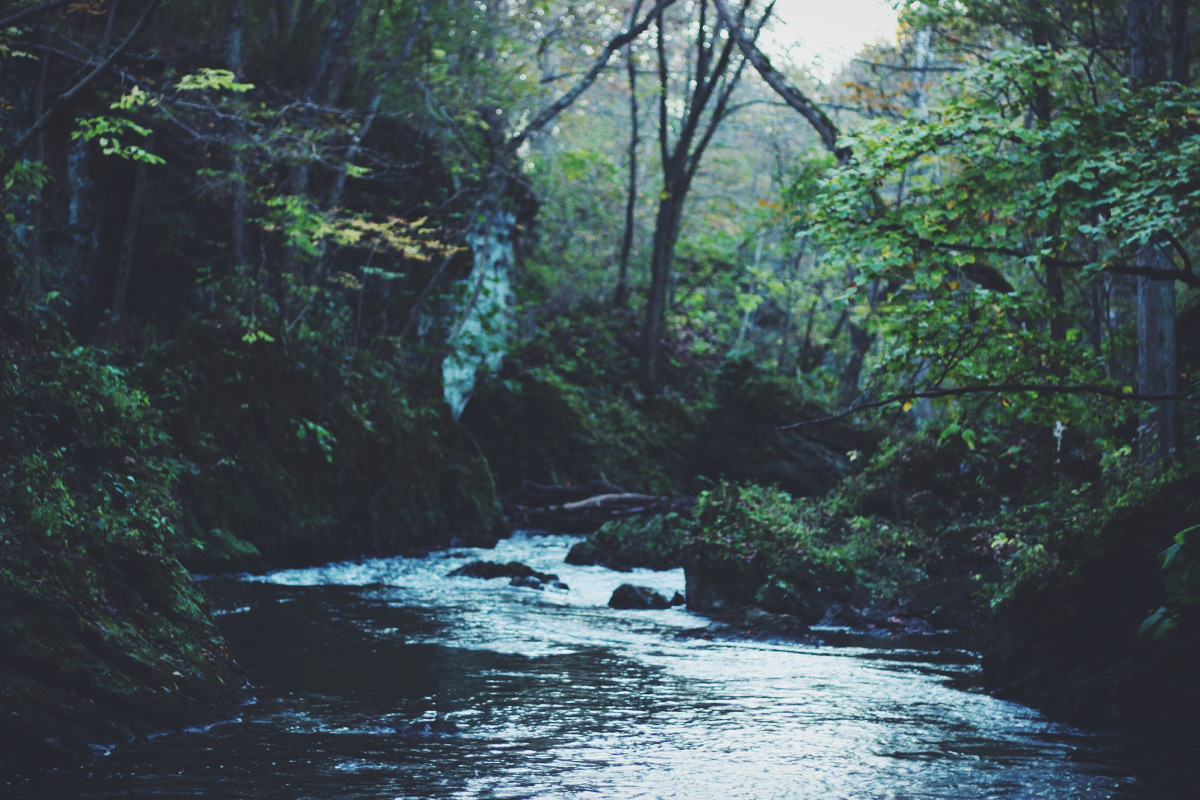
\includegraphics[width=\linewidth]{stream}
\caption{Legend (350 words max). Example legend text.}
\label{fig:stream}
\end{figure}

\begin{table}[ht]
\centering
\begin{tabular}{|l|l|l|}
\hline
Condition & n & p \\
\hline
A & 5 & 0.1 \\
\hline
B & 10 & 0.01 \\
\hline
\end{tabular}
\caption{\label{tab:example}Legend (350 words max). Example legend text.}
\end{table}

Figures and tables can be referenced in LaTeX using the ref command, e.g. Figure \ref{fig:stream} and Table \ref{tab:example}.

\end{document}